\documentclass[tikz, border=2mm]{standalone}

\usepackage{tikz}
\usetikzlibrary{calc, backgrounds, arrows.meta}

% --- CUSTOM COLORS ---
\definecolor{garnet}{HTML}{73000A}
\definecolor{predict}{HTML}{00FFFF}

\begin{document}

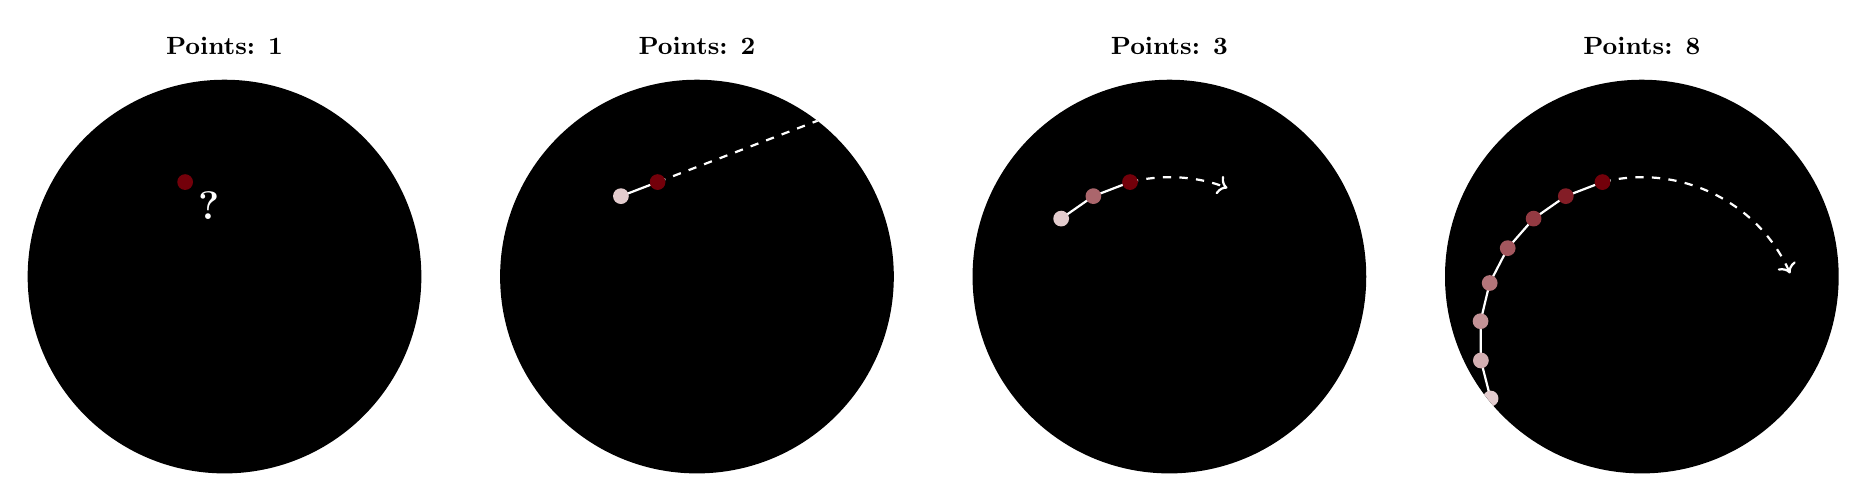
\begin{tikzpicture}

% --- MACRO: DRAW PREDICTION SCENARIO ---
% #1: X Position (Center of the scope)
% #2: Label Text (ignored)
% #3: Number of trails (N)
% #4: Prediction Type (0=None, 1=Linear, 2=Curve)
\newcommand{\drawPrediction}[4]{
    \begin{scope}[shift={(#1,0)}]
        % Background
        \fill[black] (0,0) circle (2.5cm);

        % Clipping
        \begin{scope}
            \clip (0,0) circle (2.5cm);

            % --- CURVE GEOMETRY ---
            \pgfmathsetmacro{\cx}{0}
            \pgfmathsetmacro{\cy}{-0.8}
            \pgfmathsetmacro{\hx}{-0.5}
            \pgfmathsetmacro{\hy}{1.2}

            \pgfmathsetmacro{\rad}{sqrt((\hx-\cx)^2 + (\hy-\cy)^2)}
            \pgfmathsetmacro{\thetaHead}{atan2(\hy-\cy, \hx-\cx)}

            \pgfmathsetmacro{\arcStepLen}{0.5}
            \pgfmathsetmacro{\angStep}{(\arcStepLen/\rad)*57.29578}

            % --- PREDICTION ---
            \ifnum #4=1
                % Linear (tangent)
                \pgfmathsetmacro{\prevAng}{\thetaHead + \angStep}
                \pgfmathsetmacro{\pxHead}{\cx + \rad*cos(\thetaHead)}
                \pgfmathsetmacro{\pyHead}{\cy + \rad*sin(\thetaHead)}
                \pgfmathsetmacro{\pxPrev}{\cx + \rad*cos(\prevAng)}
                \pgfmathsetmacro{\pyPrev}{\cy + \rad*sin(\prevAng)}

                \pgfmathsetmacro{\dx}{\pxHead-\pxPrev}
                \pgfmathsetmacro{\dy}{\pyHead-\pyPrev}

                \draw[white!50, dashed, thick, ->]
                    (\pxHead,\pyHead) -- ++(\dx*6,\dy*6);
            \fi

            \ifnum #4=2
                % Curved prediction
                \ifnum #3=3
                    \draw[white!50, dashed, thick, ->]
                        (\hx,\hy) arc (\thetaHead:\thetaHead-35:\rad);
                \else
                    \draw[white!50, dashed, thick, ->]
                        (\hx,\hy) arc (\thetaHead:\thetaHead-80:\rad);
                \fi
            \fi

            \ifnum #4=0
                \node[white, font=\bfseries\Large]
                    at (\hx+0.3,\hy-0.3) {?};
            \fi

            % --- HISTORY LINES ---
            \ifnum #3>1
                \pgfmathtruncatemacro{\limit}{#3-1}
                \foreach \i in {1,...,\limit} {
                    \pgfmathsetmacro{\sb}{\limit-\i}
                    \pgfmathsetmacro{\sbp}{\limit-(\i-1)}

                    \coordinate (c) at ({\cx+\rad*cos(\thetaHead+\sb*\angStep)},
                                        {\cy+\rad*sin(\thetaHead+\sb*\angStep)});
                    \coordinate (p) at ({\cx+\rad*cos(\thetaHead+\sbp*\angStep)},
                                        {\cy+\rad*sin(\thetaHead+\sbp*\angStep)});

                    \draw[white, thick] (p)--(c);
                }
            \fi

            % --- DOTS ---
            \pgfmathtruncatemacro{\limit}{#3-1}
            \foreach \i in {0,...,\limit} {
                \pgfmathsetmacro{\sb}{\limit-\i}
                \pgfmathsetmacro{\ang}{\thetaHead+\sb*\angStep}

                \pgfmathsetmacro{\px}{\cx+\rad*cos(\ang)}
                \pgfmathsetmacro{\py}{\cy+\rad*sin(\ang)}

                \ifnum #3=1
                    \fill[garnet] (\px,\py) circle (0.1cm);
                \else
                    \pgfmathsetmacro{\mix}{20+80*(\i/\limit)}
                    \fill[garnet!\mix!white] (\px,\py) circle (0.1cm);
                \fi
            }
        \end{scope}

        % Label
        \node[above, font=\bfseries\small, text=black] at (0,2.7)
            {Points: #3};
    \end{scope}
}

% --- SCENARIOS ---
\drawPrediction{-9}{}{1}{0}
\drawPrediction{-3}{}{2}{1}
\drawPrediction{3}{}{3}{2}
\drawPrediction{9}{}{8}{2}

\end{tikzpicture}

\end{document}
